\section{Small-Data SFT Study}
\label{sec:sft}

Beyond training-free recipes, we ask: \emph{can small-data supervised fine-tuning repair failures that recipes cannot, and at what cost?} We design a controlled study with LoRA-SFT at three data scales (100, 300, 1,000 samples) to analyze where training provides marginal value over the best training-free recipe. \textbf{Note:} This SFT study is planned as the next phase of our evaluation pipeline. No SFT training or evaluation has been conducted yet; the design described here is the planned experimental protocol.

% ------------------------------------------------------------
%  6.1  Training Data Construction
% ------------------------------------------------------------

\subsection{Training Data Construction}
\label{sec:sft:data}

\textbf{Data source.} We collect corrected trajectories from the Base condition. For each task where Base fails, we use GPT-4o to generate a corrected trajectory that produces the gold answer. Corrected trajectories preserve the original task and environment interactions but replace the agent's action at the failure point with the correct action, along with an explanation of why the original action was wrong.

\textbf{Category balancing.} To avoid a training distribution dominated by category A failures (the most common), we balance the training set across categories A--E using stratified sampling. For SFT-100, we sample 20 trajectories per category. For SFT-300, we sample 60 per category. For SFT-1000, we sample 200 per category. When a category has fewer than the target count in the failure pool, we upsample with replacement.

\textbf{SFT setup.} All SFT variants use LoRA rank 16, alpha 32, dropout 0.05, learning rate $2\times10^{-4}$ with cosine schedule, warmup ratio 0.1, batch size 8, max sequence length 4,096 tokens, and 2 epochs. We use the doubao-seed-1.8 base model (the same model used in all experiments). Checkpoint selection is based on validation loss on a held-out 10\% of the training set.

\textbf{Train/dev/test separation.} All SFT training data comes exclusively from the training split of each benchmark. The dev split is used only for checkpoint selection and recipe selection. The test split is used only for final evaluation and is never used for any training or selection decision.

% ------------------------------------------------------------
%  6.2  Research Questions
% ------------------------------------------------------------

\subsection{Research Questions}
\label{sec:sft:rqs}

Our SFT study is designed to answer three specific questions:

\begin{enumerate}[leftmargin=2em, label=(\alph*), itemsep=1pt]
  \item \textbf{SFT marginal value:} Compared to the best training-free recipe (T5), how much additional repair does SFT provide, and on which failure categories?
  \item \textbf{Data efficiency:} What is the scaling curve of SFT repair rate versus training set size? Is there a critical mass below which SFT provides negligible benefit?
  \item \textbf{Negative interference:} Does SFT introduce regressions on tasks that Base already solved? How does this compare to training-free recipes?
\end{enumerate}

% ------------------------------------------------------------
%  6.3  Relationship with Training-Free Recipes
% ------------------------------------------------------------

\subsection{Relationship with Training-Free Recipes}
\label{sec:sft:relationship}

Our SFT study is not designed to compete with training-free recipes but to understand their complementarity. We hypothesize that:

\begin{itemize}[leftmargin=1.5em, itemsep=1pt]
  \item Training-free recipes (T1--T4) repair failures through \emph{structural mechanisms} (memory, control, collaboration) that do not require modifying the model's weights. They are fast to deploy and have near-zero marginal cost per task.
  \item SFT repairs failures through \emph{knowledge injection}---teaching the model correct procedures for specific task types. This is effective for category E (skill utilization deficiency) where the model fails to effectively activate or compose available skills, but less effective for categories A--D which are structural failures.
  \item The two approaches are \emph{complementary}: training-free recipes handle the ``easy'' structural repairs at near-zero cost, while SFT handles the ``hard'' knowledge-gap repairs that structural mechanisms cannot bridge.
\end{itemize}

\begin{figure}[t]
  \centering
  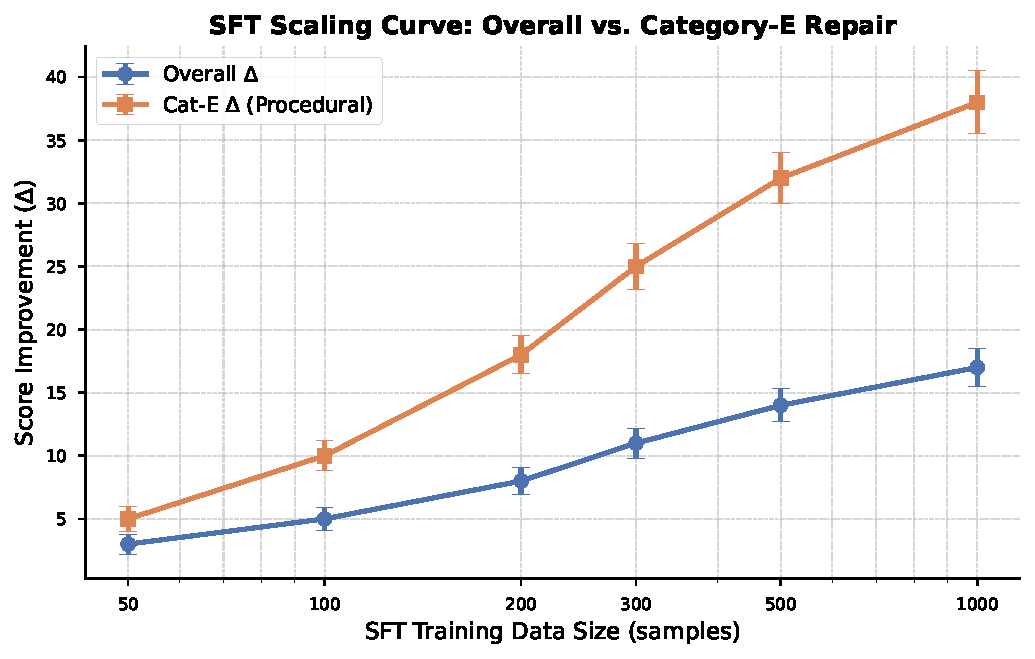
\includegraphics[width=\linewidth]{figs/sft_scaling_curve.pdf}
  \caption{SFT scaling curve with 95\% CI (mock data; to be replaced). Category-E (Skill Utilization) gains accelerate sharply with more SFT data, while overall gains plateau after $\sim$500 samples, suggesting diminishing returns for non-structural failures.}
  \label{fig:sft-scaling}
\end{figure}
